
\begin{frame}{Functional sensitivity: other paths \citep{gustafson:1996:local}}

For $\p(\nuk \vert \phi)$, we used a multiplicative perturbation.

\vspace{1em}

\begin{mdframed}[style=MyFrame]
\begin{center}
{\bf Could we have used other paths through function space? }
\end{center}
\end{mdframed}

\pause

%Recall that we used $\p(\nuk \vert \phi) \propto \pbase(\nuk)\exp(\phi(\nuk))$.
Consider, for example, ``mixture distributions'':
%
\begin{align*}
\p(\nu \vert \phi_{mix}) \propto{}
\pbase(\nu) + \phi_{mix}(\nu)
\quad\textrm{and}\quad
\phi_{mix}(\nu) = \palt(\nu) - \pbase(\nu)
\end{align*}

\vspace{-0.5em}
Then $\t\mapsto \p(\nu \vert t\phi_{mix})$ also parameterizes a path from
$\pbase$ to $\palt$.

\pause

\vspace{-0.5em}
\begin{figure}[!h]
\centering
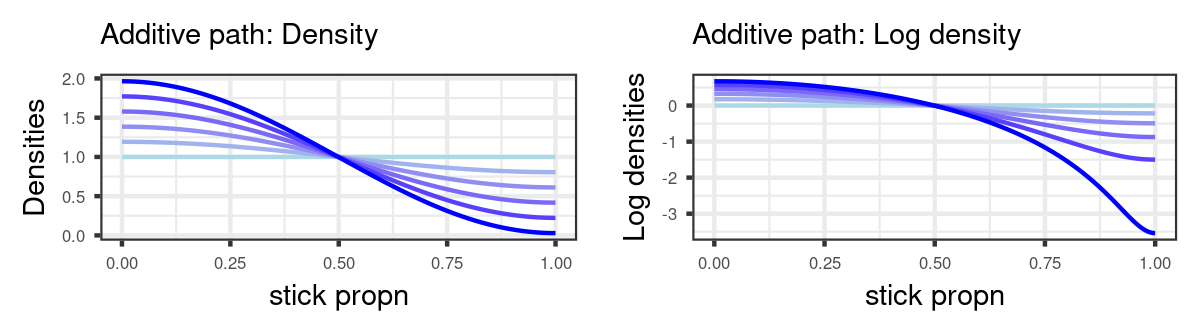
\includegraphics[width = 0.8\paperwidth]{./figure/lin_path-1.png}
%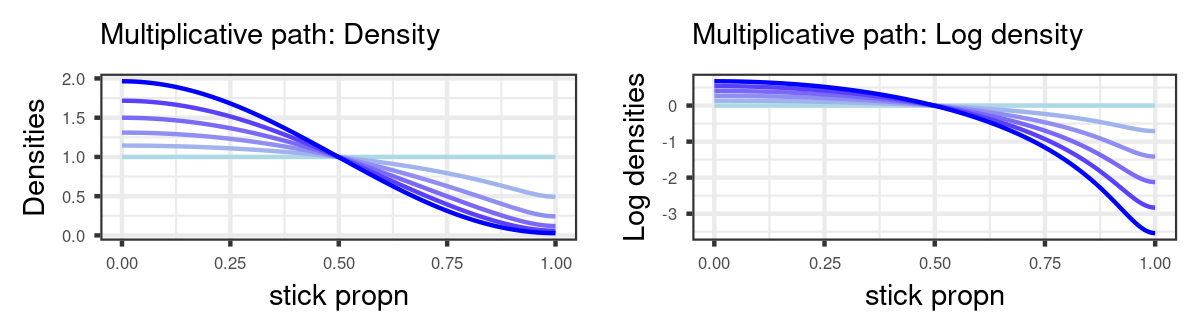
\includegraphics[width = 0.7\paperwidth]{./figure/mult_path-1.png}
\end{figure}
%
%\vspace{-1.5em}

\pause

{\centering
{\bf Question:} Is there anything wrong with using $\phi_{mix}$ with our VB approximation?
}
\end{frame}




\begin{frame}{Functional Sensitivity: Other Paths}

% \textbf{Proposition (c.f. \citet{gustafson:1996:local})}

% If $\norm{\phi_{mix}}_1 := \int_0^1 \abs{\phi_{mix}(\nu)} d\nu$ is small, then
% $\p(\nu \vert \phi_{mix})$ can be normalized.

% If $\p(\nu \vert \phi_{mix})$ can be normalized, then $\norm{\phi_{mix}}_1 < \infty$.

% \pause

% $\Rightarrow$ $\norm{\cdot}_1$ is the sensible norm for mixture perturbations.

\pause

\textbf{Theorem 3.} (Differentiability of other paths.)

\pause 

Let
$S_{mix} := \{\phi_{mix}: \phi_{mix} =
 \palt - \pbase \textrm{ for some density }
 \palt \ll \pbase \}$.

\pause 

For any $\phi_{mix} \in S_{mix}$, the conditions of 
Theorem 1 are satisfied under some additional mild integrability
assumptions on $\q_\eta$.  So the map $\t \mapsto \etaopt(\t \phi_{mix})$
is continuously differentiable.

\pause

But normalizability of $\p(\nu \vert \phi_{mix})$ is determined by
$\norm{\phi_{mix}}_1$, and the error of the derivative is
arbitrarily large in any $\norm{\cdot}_1$-neighborhood of the zero function.

\pause

$\Rightarrow$ No extension
of $S_{mix}$ to $\lp{1}$ of the map $\phi_{mix} \mapsto \etaopt(\phi_{mix})$ 
can be Fr{\'e}chet differentiable. 

% ...and the map
% $\phi_{mix} \mapsto \KL{\etaopt, \phi_{mix}}$ is discontinuous
% in $\norm{\cdot}_1$ on $S_{mix}$.

% Fr{\'e}chet differentiability implies
% continuity.  Consequently, no extension
% of $S_{mix}$ to $\lp{1}$ of the map $\phi_{mix} \mapsto \etaopt(\phi_{mix})$ 
% can be Fr{\'e}chet differentiable.  

\hfill $\square$

\pause

\textbf{Note:}
An analogous result holds for all $\lp{p}$ spaces with $p < \infty$.

\end{frame}






\begin{frame}{Functional Sensitivity: Other Paths}

{\bf What went wrong with the mixture distribution?}

\begin{minipage}{0.49\textwidth}
\onslide<2->{
These red and blue densities are
\begin{itemize}
    \item Distant in KL and $\norminf{\cdot}$, but
    \item Close in $\norm{\cdot}_p$ when $p < \infty$.
\end{itemize}
}

\onslide<3->{
\vspace{1em}
A parameterization + prior normalizability dictates a norm.
}

\onslide<4->{
\vspace{1em}
For differentiability of $\etaopt$, the norm's topology must match that of KL.
}

\onslide<5->{
\vspace{1em}
$\Rightarrow$ {\bf We consider only multiplicative perturbations for VB.}
}

%
\end{minipage}
%
% Figure minipage
\begin{minipage}{0.49\textwidth}
\onslide<2->{
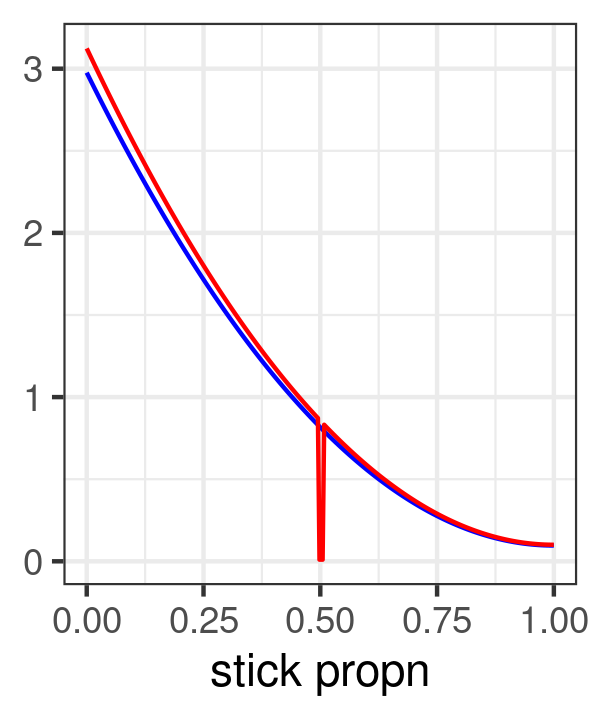
\includegraphics[width=1.0\linewidth,height=1.176\linewidth]{figure/func_dist-1} 
}
\end{minipage}

\end{frame}

